\documentclass[a4paper,12pt]{article}

\usepackage[
    left=2cm,
    right=2cm,
    top=3cm,
    bottom=3cm
]{geometry}

\usepackage[utf8]{inputenc}
\usepackage[czech]{babel}
\usepackage[T1]{fontenc}
\usepackage{graphicx}
\usepackage{array}
\usepackage{booktabs}
\usepackage{tabularx}
\usepackage{makecell}
\usepackage{float}
\usepackage{newunicodechar}
\usepackage{url}
\usepackage{siunitx}
\usepackage{listings}
\usepackage{xcolor}
\usepackage{diagbox}
\usepackage{hyperref}
\usepackage{tikz}
\usepackage{pgfplots}
\pgfplotsset{compat=1.18}

\usepackage{fancyhdr}
\pagestyle{fancy}

\fancyhf{}
\fancyhead[L]{Spektrometrie ve viditelném spektru}
\fancyhead[R]{Pavel Pernička}
\fancyfoot[C]{\thepage}

\fancypagestyle{firstpage}{
    \fancyhf{}
    \renewcommand{\headrulewidth}{0pt}
    \renewcommand{\footrulewidth}{0pt}
    \fancyfoot[C]{\thepage}
}

\definecolor{myblue}{RGB}{111,0,248}
\newcommand{\colorcircle}[1]{%
  \tikz[baseline=-0.6ex]\draw[fill=#1,draw=none] (0,0) circle (1.5ex);%
}
\newcommand{\unitC}{\,^\circ\mathrm{C}}
\newcommand{\unitV}{\,\mathrm{V}}
\newcommand{\unitA}{\,\mathrm{A}}
\newcommand{\units}{\,\mathrm{s}}
\newcommand{\unitmin}{\,\mathrm{min}}

\newcommand{\centered}[1]{\begin{tabular}{l} #1 \end{tabular}}

\addto\captionsczech{\renewcommand{\refname}{Seznam použité literatury}}
\addto\captionsczech{\renewcommand{\figurename}{\textbf{Obrázek}}}
\addto\captionsczech{\renewcommand{\tablename}{\textbf{Tabulka}}}
\renewcommand{\lstlistingname}{\textbf{Kód}}

\lstset{
    language=Python,
    basicstyle=\ttfamily\footnotesize,
    keywordstyle=\color{blue},
    commentstyle=\color{gray},
    stringstyle=\color{red},
    numbers=left,
    numberstyle=\tiny\color{gray},
    stepnumber=1,
    breaklines=true,
    frame=single
}

\begin{document}
\thispagestyle{firstpage}

\vspace*{\fill}
\begin{center}
\renewcommand{\arraystretch}{1.75}

\begin{tabularx}{\textwidth}{|X|X|X|}
    \hline
    \multicolumn{1}{|c|}{\rule{0pt}{2.25cm} 
\includegraphics[height=2cm]{img/ctu_logo.png}}
    & \multicolumn{2}{c|}{\makecell{\textbf{KATEDRA FYZIKY}}} \\
    \hline
    \multicolumn{3}{|c|}{\Large \textbf{\centered{LABORATORNÍ CVIČENÍ Z FEN}}} \\
    \hline
    \multicolumn{2}{|X}{\small{Jméno} \newline \textbf{Pavel Pernička}}
    & \multicolumn{1}{|X|}{\small{Datum měření} \newline \textbf{5.11.2025}} \\
    \hline
    {\small{Semestr} \newline \textbf{Zimní 2025}}
    & {\small{Ročník} \newline \textbf{2.}}
    & {\small{Datum odevzdání} \newline \textbf{16.1.2026}} \\
    \hline
    \multicolumn{3}{|c|}{\rule{0pt}{1cm}} \\
    \hline
    \multicolumn{1}{|X|}{\small{Číslo úlohy \newline \textbf{1}}}
    & \multicolumn{2}{|p{9cm}|}{\small{Název úlohy \newline \textbf{Spektrometrie ve viditelném spektru}}} \\
    \hline
\end{tabularx}

\end{center}
\vspace*{\fill}

\newpage
\section{Úkol měření}
\begin{itemize}
    \item Určete spektra jednotlivých spektrálních lamp a dalších vzorků, vykreslete grafy.
\end{itemize}


\section{Seznam použitých přístrojů}
\begin{itemize}
    \item Spektrometr
    \item Kamera pro snímání spektra
    \item Držák pro lampy
    \item Spektrální lampy -- Zinek, Neon, Sodík, Rtuť, Helium
    \item Další zdroje pro určení spektra -- LED světlo na mobilu, klasická žárovka
\end{itemize}

\section{Postup měření}
\begin{itemize}
    \item Do patice v držáku před škvírou spektrometru pro vstup světla vložíme spektrální lampu.
    \item Zapneme napájení lampy a počkáme chvíli, než se rozžhaví.
    \item V programu pozorujeme stream z kamery, která je namířená na výstupní škvíru spektrometru.
    \item Nastavíme parametry expozice jednotlivých snímků z kamery tak, abychom viděli spektrum co nejjasněji.
    \item Až jsme se snímkem spokojeni, uložíme jej ve formátu \textit{.tiff}.
\end{itemize}

\section{Teorie}
\subsection{Fyzikální princip}
Spektrální lampy, pro které měříme spektra jsou plynové výbojky plněné určitým prvkem. Průchodem proudu trubicí výbojky vzniká stabilní výboj
a atomy prvku jsou excitovány. To znamená, že elektrony v atomovém obalu se nacházejí ve vyšších energetických hladinách, což je ale nestabilní stav s typickou životností okolo $10^{-9}$ až $10^{-8}\ s$. 
Následně se elektron vrací do nižšího energetického stavu a vyzařuje foton o energii $E_{vyšší} - E_{nižší} = h\nu = \frac{hc}{\lambda}$. 

Jejikož ale existují zakázané přechody mezi hladinami, kde je pravděpodobnost přechodu velmi malá, tak ve spektru vyzářených fotonů vidíme zastoupené pouze určité vlnové délky, které se projeví právě spektrálními čarami po průchodu spektrometrem. 

\subsection{Spektrometr}
Spektrometr obecně funguje na principu převedení vstupního záření do rovnoběžného svazku pomocí čočky a následné disperzi pomocí optické mřížky či hranolu. 

Při práci na této laboratorní úloze byl použit sovětský laboratorní spektrometr \textit{UF-90}, který je prizmatický, tedy používá k disperzi optický hranol a soustavu zrcadel a čoček. 

\newpage
\section{Naměřená data}
Pomocí kamery jsme vytvořili snímky různých světelných zdrojů, které vypadají následovně:

\begin{center}
\setlength{\tabcolsep}{6pt}
\renewcommand{\arraystretch}{1.5}

\begin{tabularx}{\textwidth}{XXX}

\begin{minipage}{\linewidth}
\centering
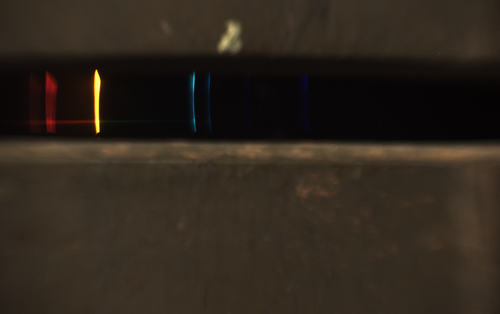
\includegraphics[width=\linewidth]{img/photos/helium.png}
\par\small Výbojka – helium
\end{minipage}
&
\begin{minipage}{\linewidth}
\centering
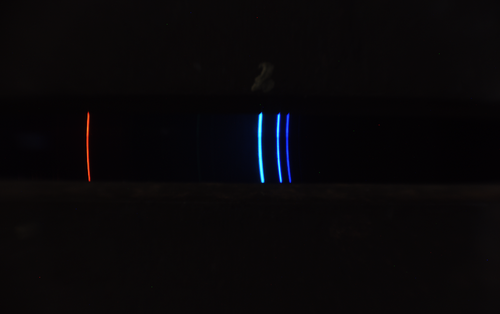
\includegraphics[width=\linewidth]{img/photos/zn.png}
\par\small Výbojka – zinek
\end{minipage}
&
\begin{minipage}{\linewidth}
\centering
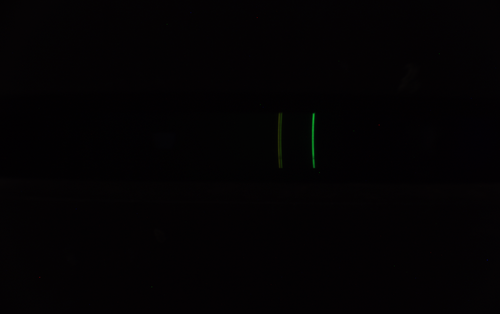
\includegraphics[width=\linewidth]{img/photos/hg_chladna.png}
\par\small Výbojka – rtuť (studená)
\end{minipage}
\\[60pt]

\begin{minipage}{\linewidth}
\centering
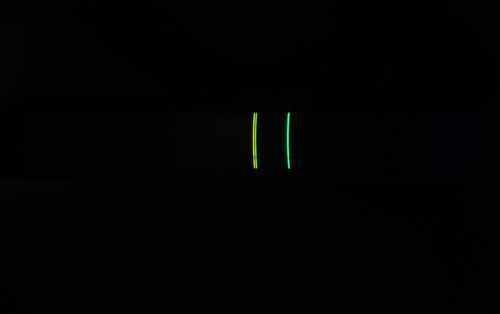
\includegraphics[width=\linewidth]{img/photos/hg_zahrata.png}
\par\small Výbojka – rtuť (zahřátá)
\end{minipage}
&
\begin{minipage}{\linewidth}
\centering
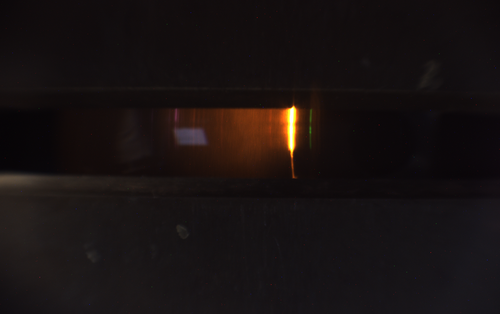
\includegraphics[width=\linewidth]{img/photos/na.png}
\par\small Výbojka – sodík
\end{minipage}
&
\begin{minipage}{\linewidth}
\centering
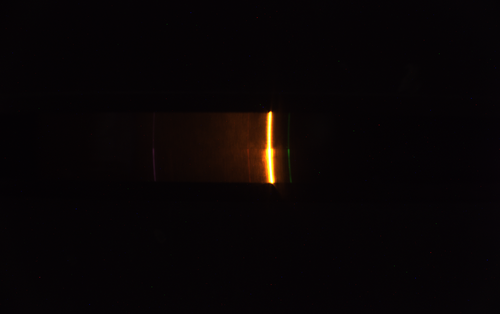
\includegraphics[width=\linewidth]{img/photos/na_zahrata.png}
\par\small Výbojka – sodík (zahřátá)
\end{minipage}
\\[60pt]

\begin{minipage}{\linewidth}
\centering
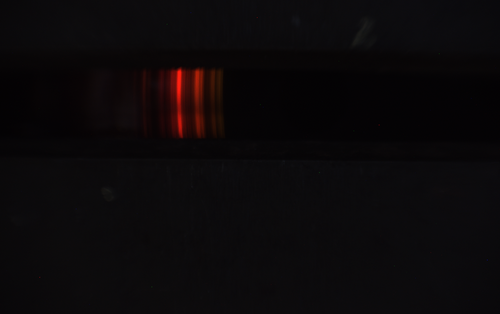
\includegraphics[width=\linewidth]{img/photos/neon106.png}
\par\small Výbojka – neon
\end{minipage}
&
\begin{minipage}{\linewidth}
\centering
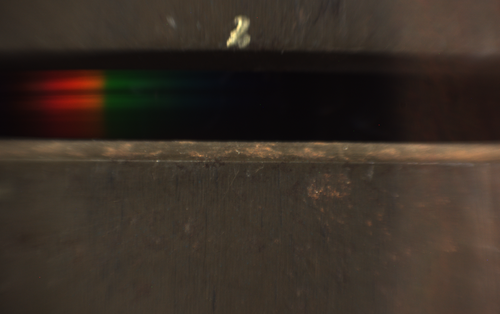
\includegraphics[width=\linewidth]{img/photos/zarovka.png}
\par\small Žárovka
\end{minipage}
&
\begin{minipage}{\linewidth}
\centering
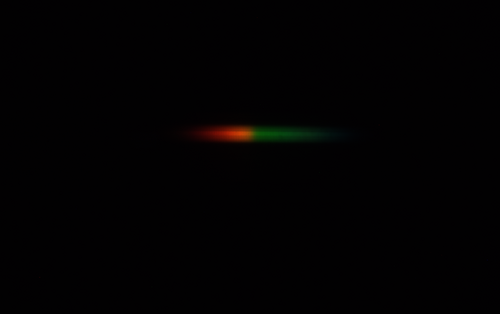
\includegraphics[width=\linewidth]{img/photos/mobil.png}
\par\small LED
\end{minipage}
\\

\end{tabularx}
\end{center}

Jak jsme očekávali v teoretickém úvodu, na snímcích spektra jednoprvkových výbojek vidíme několik diskrétních spektrálních čar v různé kvalitě. U vzorku klasické žárovky a LED světla vidíme v určité oblasti spojitá spektra.

\section{Zpracování naměřených dat}
Abychom z bitmapové fotografie spektra získali spektrogram, tedy graf závislosti intenzity záření na vlnové délce, budeme potřebovat specializovaný software. Tento software si napíšeme sami za použití programovacího jazyku Python. 

Na počátku samotného řetězce operací bude vstupní \textit{.tiff} obrázek vyfoceného spektra. Jelikož použitá kamera je přizpůsobena pro snímání v RGB barvách a tím pádem obsahuje Bayerův filtr, který propouští určité části spektra do určitých fotobuněk senzoru a výsledné hodnoty se určují interpolací, nemůžeme se na dané barvy spolehnout, protože do sebe částečně vzájemně prosakují. 
Proto v prvním kroku snímek převedeme na černobílý, kde bude bude jednokanálová normovaná intenzita dopadajícího světla funkcí souřadnic snímku. 

Spektrální čáry se ale nacházejí v nějaké linii, takže dalším stupněm bude transformace 2-dimensionálního snímku do 1D pole podél určité linie. Abychom zamezili zkreslení šumem, kolem zvolené linie vezmeme pruh určité šířky, přes který průměrujeme hodnoty. 
Na 1D hodnoty aplikujeme drobné vyhlazení pomocí klouzavého průměru a následně detekujeme peaky pomocí hledání lokálních maxim. 

\begin{figure}[H]
\centering

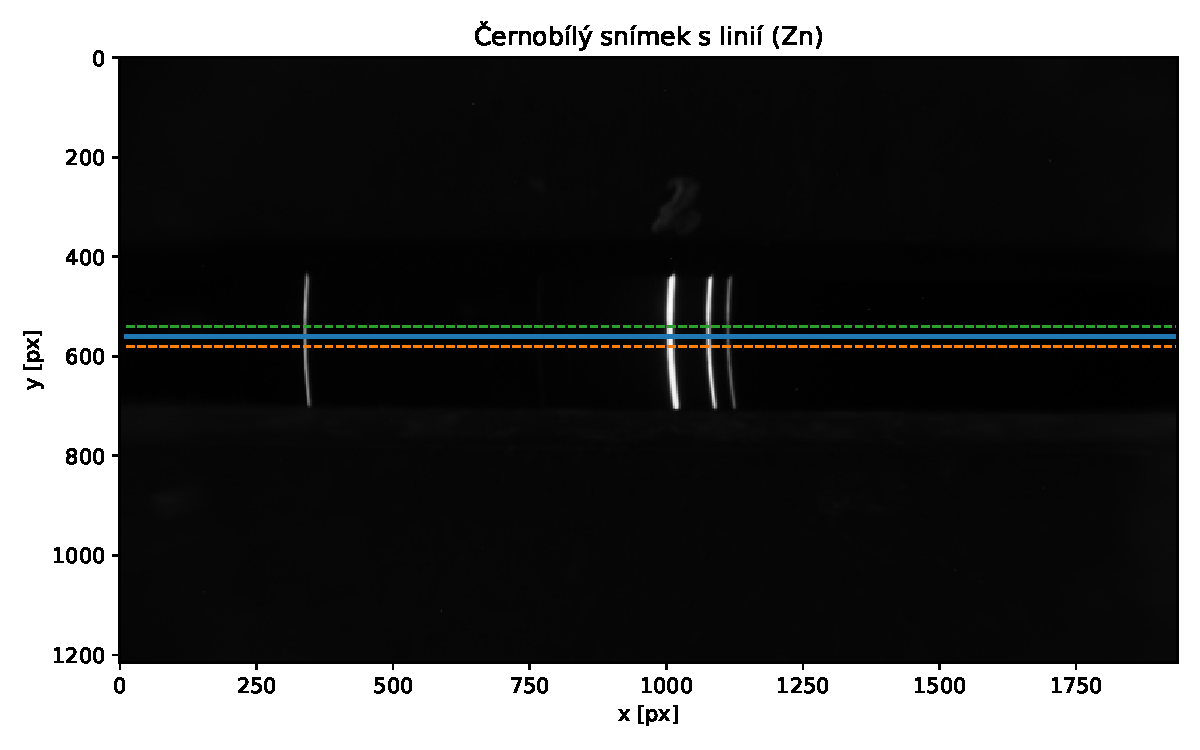
\includegraphics[width=0.90\textwidth]{img/charts/zn_line.pdf}

\vspace{10pt}

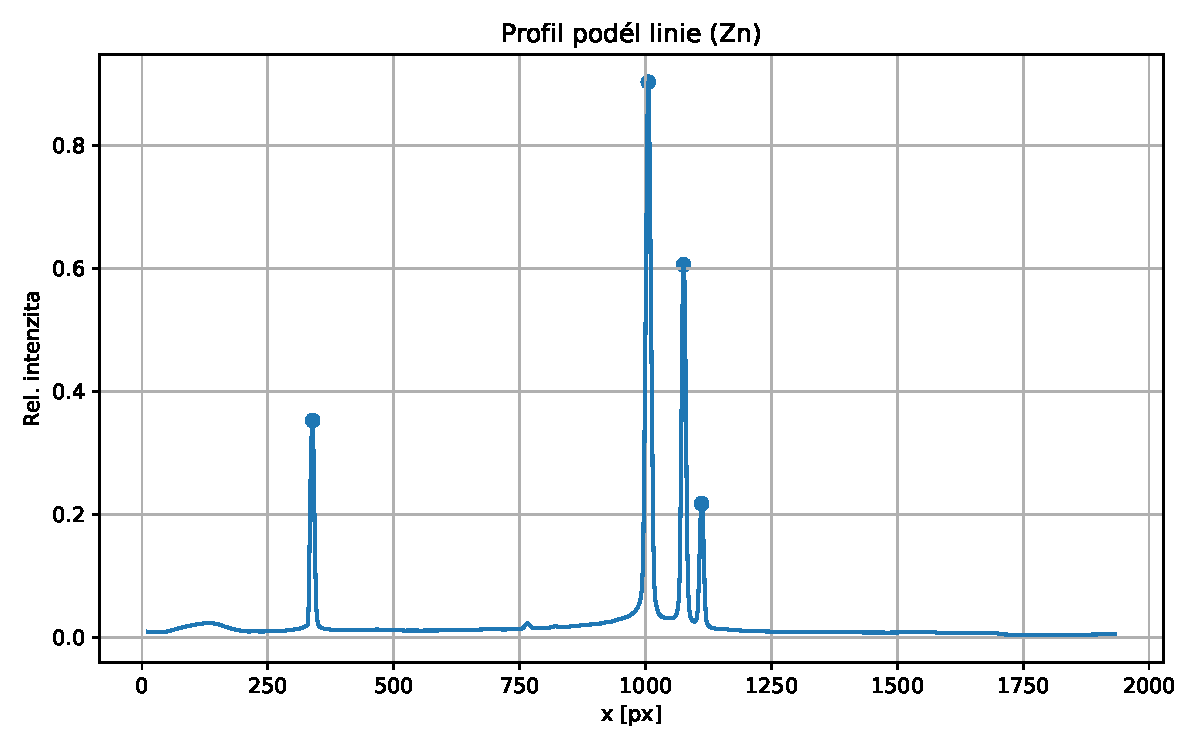
\includegraphics[width=0.90\textwidth]{img/charts/zn_profile.pdf}

\caption{Zpracování spektra zinkové výbojky: Černobílý obrázek s vyznačenou linií průzkumu spektra a spektrum $I(x)$.}
\label{fig:zn_processing}
\end{figure}

\newpage
Nyní máme spektrum $I(x)$ a z něj chceme dostat $I(\lambda)$. To provedeme kalibrací pomocí známého vzorku se známými vlnovými délkami spektrálních čar. Tedy na nelezené maxima namapujeme vlnové délky a závislost proložíme polynomen $n$-tého řádu.
Jelikož pracujeme na krátkém úseku spektra, můžeme použít lineární aproximaci. Pokud kalibraci aplikujeme na ten samý vzorek zinku, dostaneme obrázek \ref{fig:zn_spectrum}.

\begin{figure}[H]
\centering
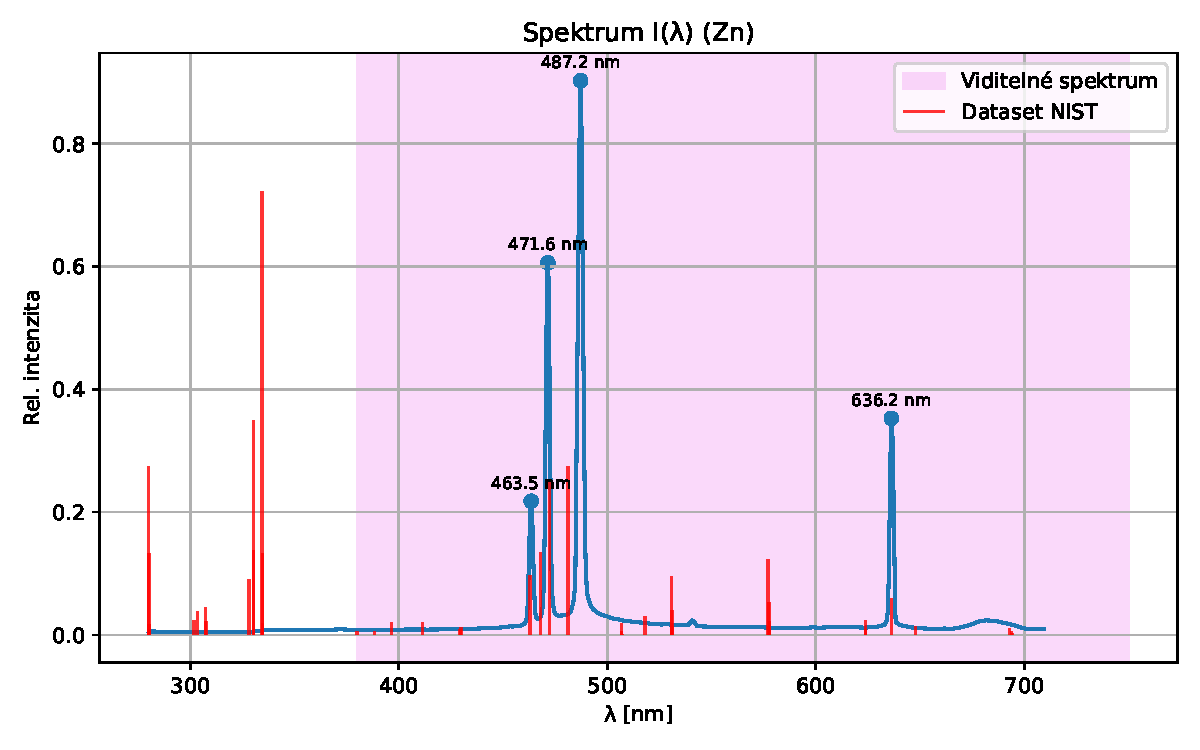
\includegraphics[width=0.95\textwidth]{img/charts/zn_spectrum.pdf}
\caption{Získané spektrum zinkové výbojky.}
\label{fig:zn_spectrum}
\end{figure}

\newpage
\section{Srovnání spekter}
Pro srovnání použijeme data z NIST datasetu \cite{nist}, které vyneseme do našeho laboratorně naměřeného spektrogramu. 

\begin{figure}[H]
\centering
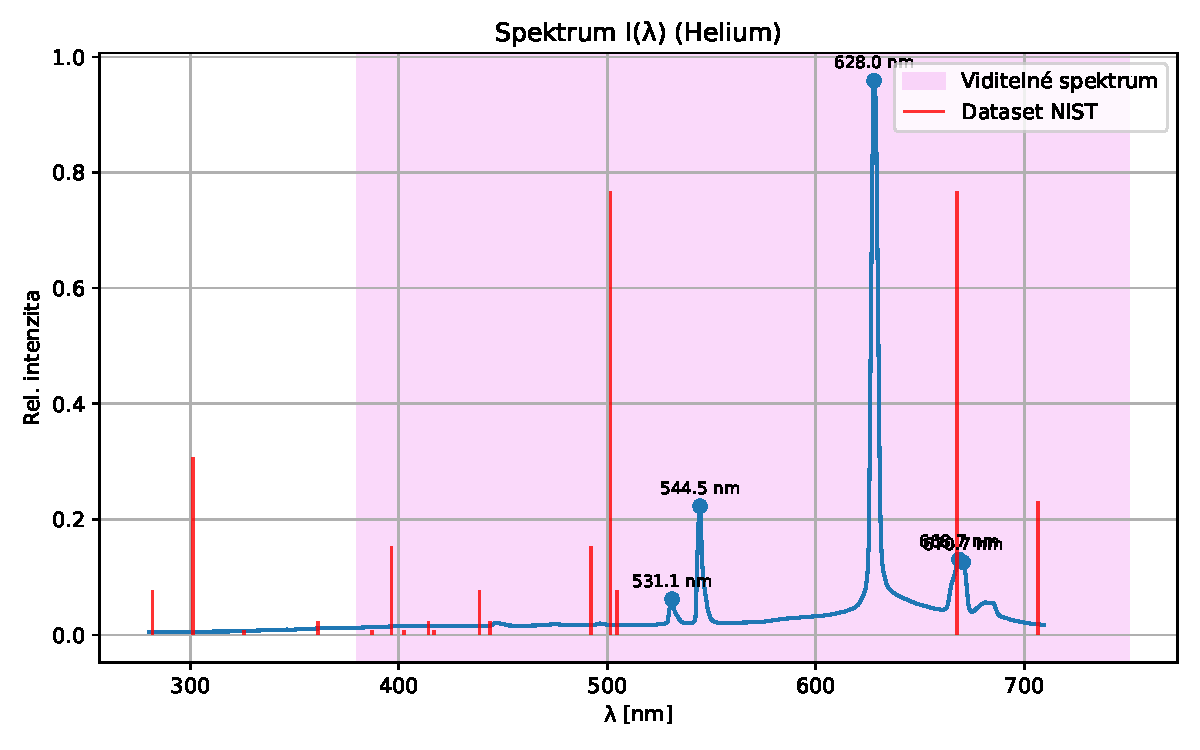
\includegraphics[width=0.85\textwidth]{img/charts/helium_spectrum.pdf}
\caption{Spektrum helia}
\label{fig:he}
\end{figure}

\begin{figure}[H]
\centering
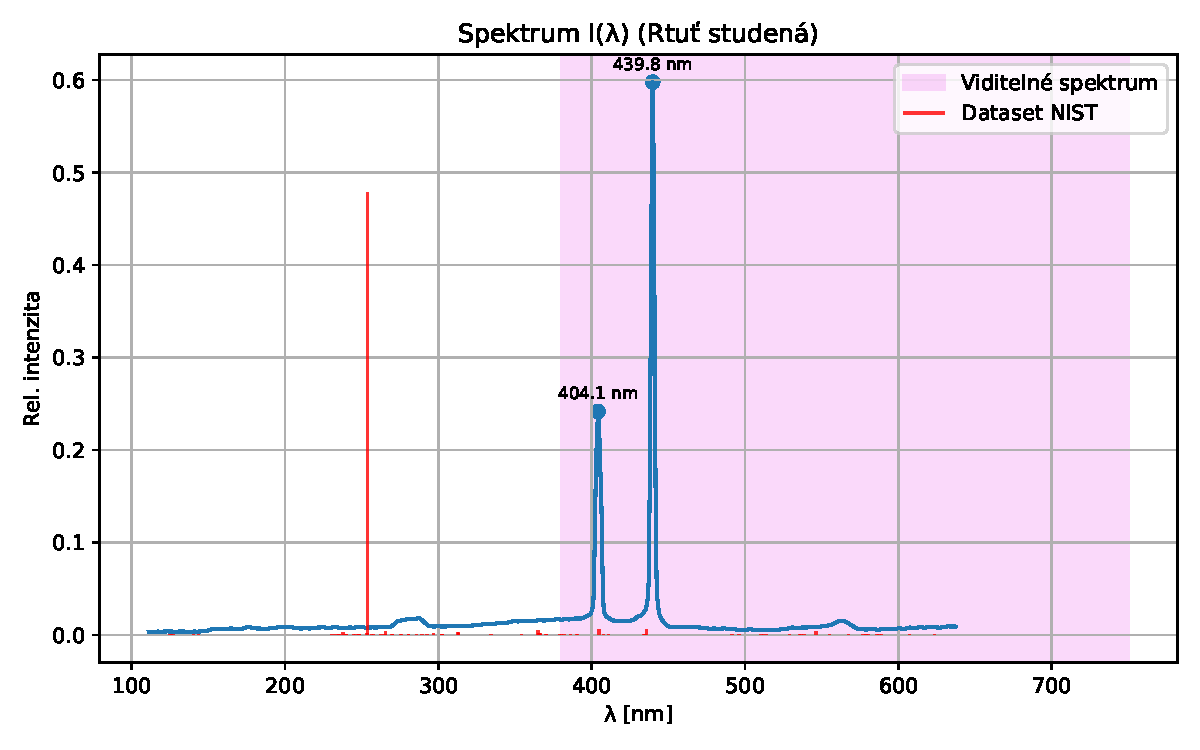
\includegraphics[width=0.85\textwidth]{img/charts/hg_chladna_spectrum.pdf}
\caption{Spektrum neohřáté rtuťi}
\label{fig:hg_cold}
\end{figure}

\begin{figure}[H]
\centering
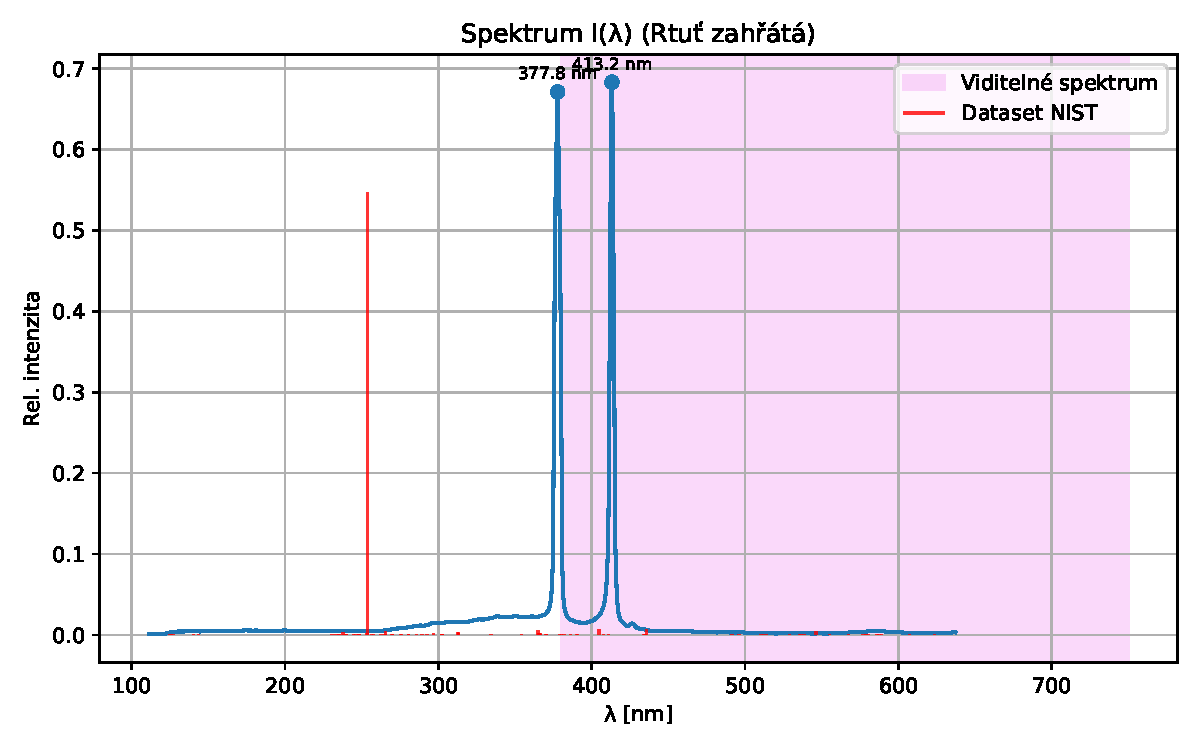
\includegraphics[width=0.90\textwidth]{img/charts/hg_zahrata_spectrum.pdf}
\caption{Spektrum ohřáté rtuťi}
\label{fig:hg_warm}
\end{figure}

\begin{figure}[H]
\centering
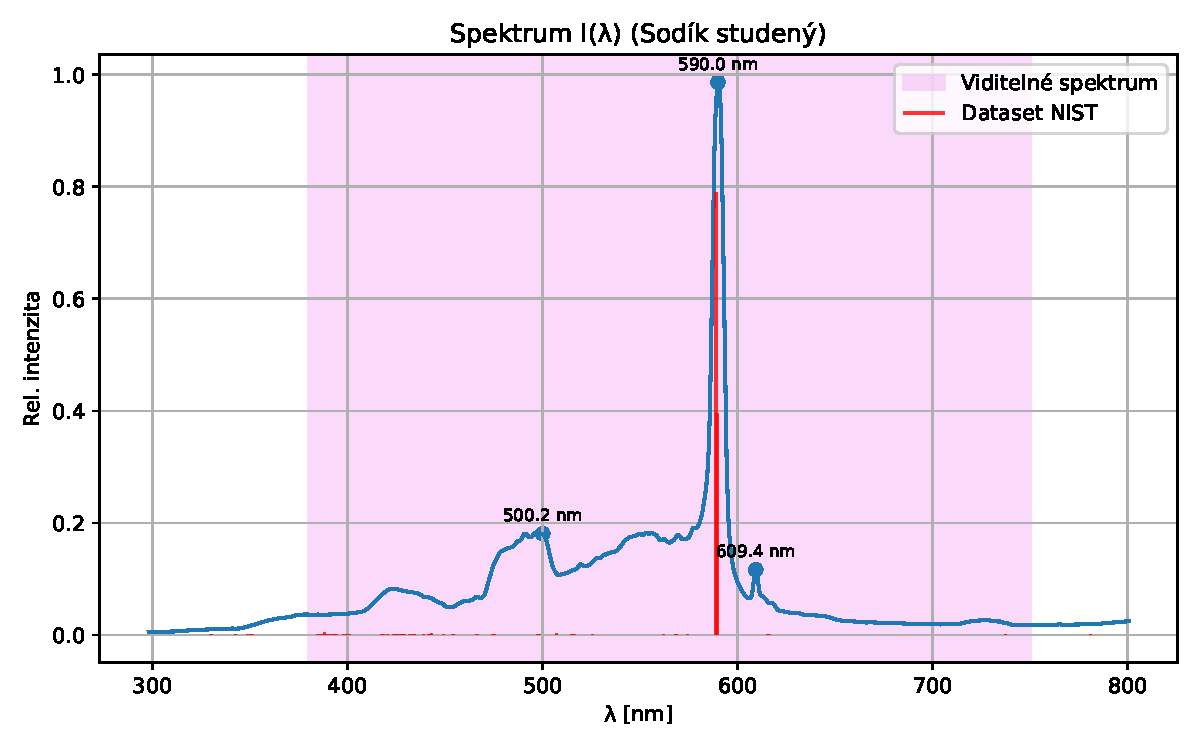
\includegraphics[width=0.90\textwidth]{img/charts/na_spectrum.pdf}
\caption{Spektrum neohřátého sodíku}
\label{fig:na_cold}
\end{figure}

\begin{figure}[H]
\centering
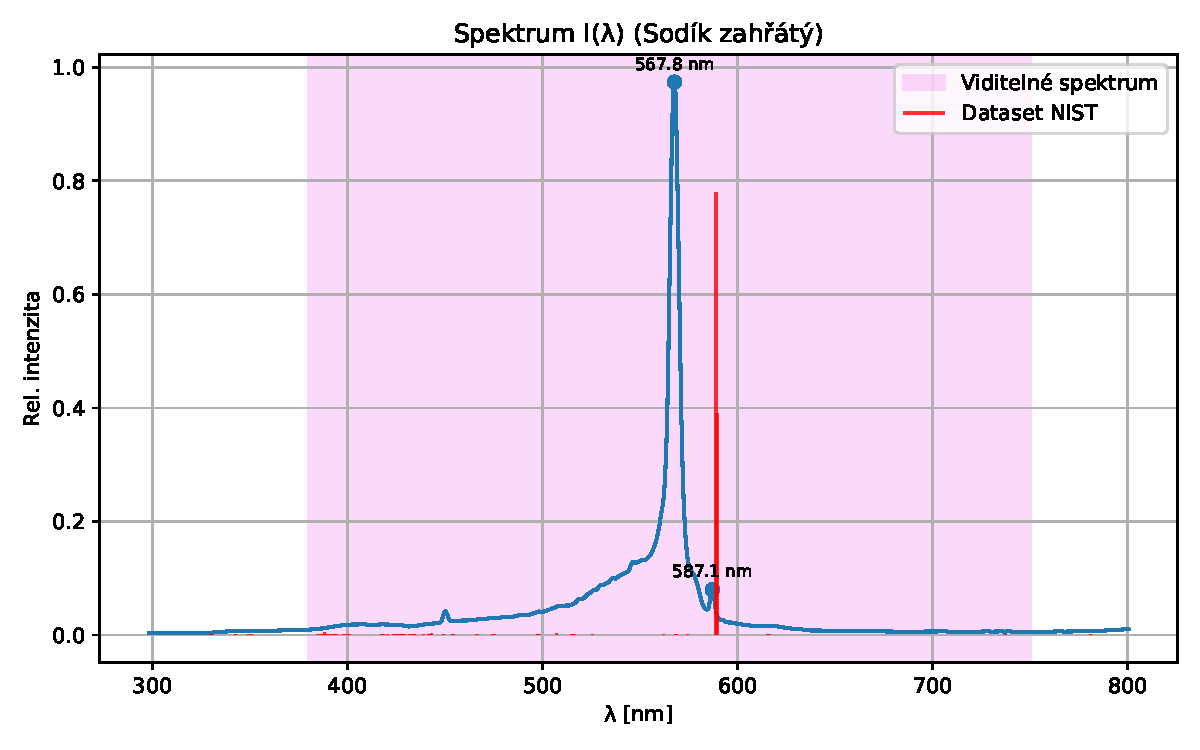
\includegraphics[width=0.90\textwidth]{img/charts/na_zahrata_spectrum.pdf}
\caption{Spektrum ohřátého sodíku}
\label{fig:na_warm}
\end{figure}

\begin{figure}[H]
\centering
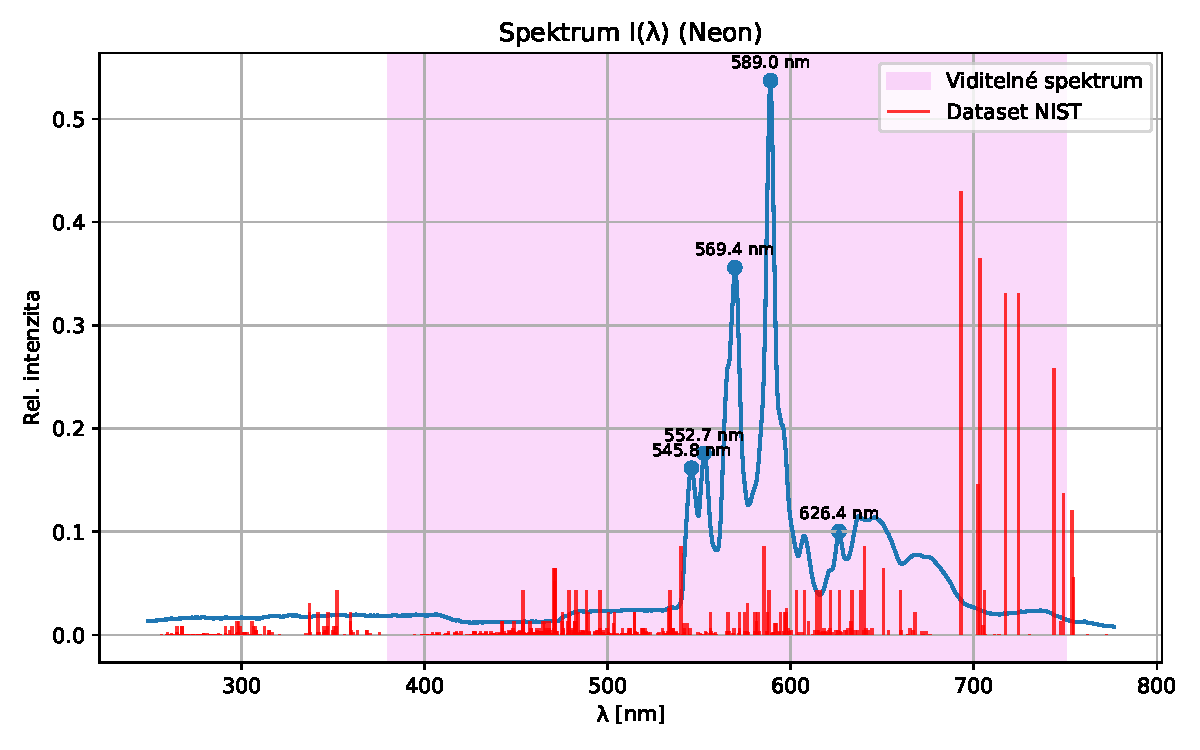
\includegraphics[width=0.90\textwidth]{img/charts/neon106_spectrum.pdf}
\caption{Spektrum neonu}
\label{fig:ne}
\end{figure}

\begin{figure}[H]
\centering
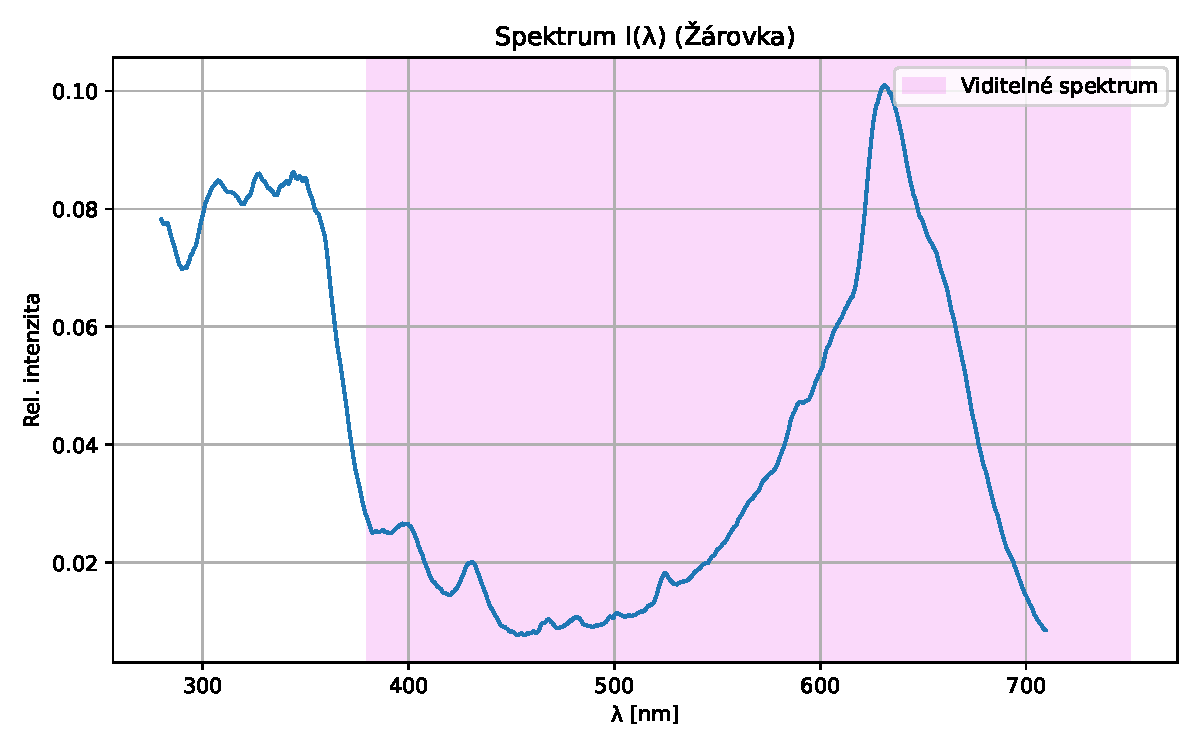
\includegraphics[width=0.90\textwidth]{img/charts/zarovka_spectrum.pdf}
\caption{Spektrum běžné žárovky}
\label{fig:zarovka}
\end{figure}

\begin{figure}[H]
\centering
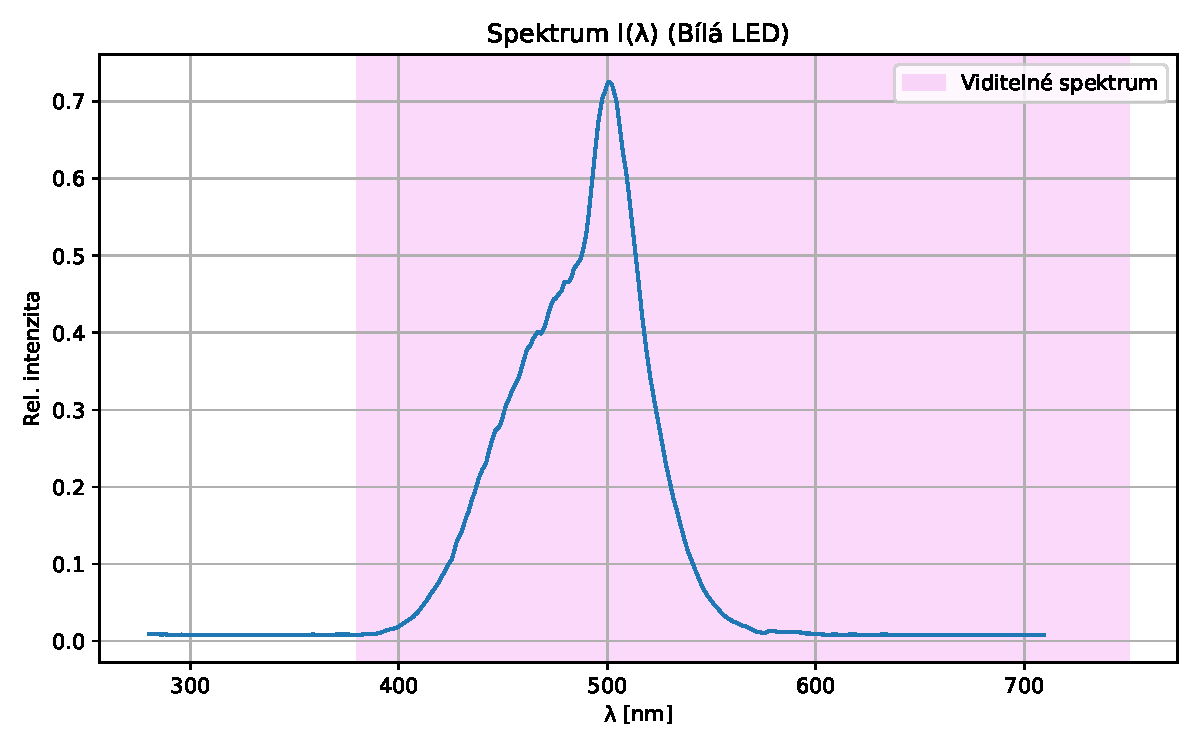
\includegraphics[width=0.90\textwidth]{img/charts/mobil_spectrum.pdf}
\caption{Spektrum bílé LED diody}
\label{fig:led}
\end{figure}

\section{Závěr}
Pomocí spektrometru a softwarového processingu snímků z něj jsme vytvořili spektrogramy jednotlivých světelných zdrojů. Pro kalibraci jsme využili známé vlnové délky spektrálních čar jednoho ze vzorků, které bohužel i tak nepříliš dobře pasovaly na naměřený vzorek. Navíc kvůli neopatrnosti měření nám u několika vzorků došlo k posunu kamery a tím pádem jsou spektra posunutá, jelikož nedošlo k opětovné kalibraci. 
Naměřená spektra jsou tedy vhodná jen na velmi hrubé odhady složení vzorků, nikoliv k přesnému určení vlnových délek spektrálních čar.

\section{Přílohy}
\begin{itemize}
    \item Python notebook se zpracováním dat
    \item Python moduly pro analýzu spektra z obrázků
    \item Snímky spektrálních čar
\end{itemize}

\begin{thebibliography}{}

    \bibitem{zadani}
    Jakub Cikhardt, Pavel Kubeš. \textit{Prezentace k předmětu Fyzika pro elektroenergetiku}. 2025.

    \bibitem{skripta}
    Michal Bednařík. \textit{Studijní texty k předmětu Fyzika 2}.
    
    \bibitem{nist}
    A.~Kramida, Yu.~Ralchenko, J.~Reader, NIST ASD Team.
    \textit{NIST Atomic Spectra Database (ver. 5.12)}.
    National Institute of Standards and Technology, Gaithersburg, MD, 2024.
    Dostupné online: \url{https://physics.nist.gov/asd}. [cit. 14.~1.~2026].

\end{thebibliography}

\end{document}
